\chapter{Testing}

	This section describes the approach to testing undertaken throughout the project, along with some results from the tests that where undertaken.

\section{Overall Approach to Testing}
	To develop the server side element of the project the programmer followed a test driven approach utilising the red-green-refactor principle.  By doing this it enabled the code to be as efficient as possible whilst still undertaking the task that block of code was expected to do. This method was chosen as the majority of the code required on the server side application didn't utilise a GUI and benefited from a much more pragmatic  approach to testing. As part of the server element had to pull in information from external sources `WebMock' was used to mock HTTP connections to the external API's, this was used to serve test data to the code and to be able to check any transformations on the data. 

	To develop the mobile application a more behaviour driven approach was used, by writing the code and conducting  a manual test seemed the more logical way. As most of the code was by use of target-action concept, meaning that the bulk of code was methods to be ran when a particular button is selected in the GUI. This also helped with the requirement testing, by ensuring that the requirements where in place and functioning on the mobile device itself. 
	
\section{Automated Testing}
	To conduct the automated tests on the server element of the project I used RSpec which is a testing environment for Ruby. RSpec has a version that's designed for the use within Ruby on Rails of which is the version used, RSpec gives the programmer the ability to test all aspects of the code including models, controllers and views. The programmer first wrote the tests that where needed for a particular feature or element of the program, and then implemented the function. However sometimes the test needed to be reviewed to ensure that it was testing the code correctly as, occasional odd results would appear after implementing a feature. 

\subsection{Stress Testing}
	Stress testing the server side element is pretty irrelevant due to the nature of the cloud based server it's running on we almost have unlimited resources to utilise if the server comes under significant stress. Heroku gives you the ability to add and remove physical resources such as CPU power and RAM whenever the demand is so high it's required. With the current scale of the application there is plenty of leeway to supply to the potential demand. If this demand became more persistent then it would be an adequate time to ensure the code is running as leanly as possible. 

	XCode 5 gives some great tools to be able to visualise how well the application is running on the mobile device, these include being able to see the current CPU and RAM usage the application is currently utilising. This data has been collated and used as part of the stress testing, currently the application only loads a certain number of events and so this is the maximum it will need to handle. However this number could go up as the server application builds a larger dataset of events, for this reason the resources used need to be as low as possible. Figures \ref{fig:iosResources} shows the resources that's in use throughout the use of the application, as you can see this is a low number. The stress test was tested on a mid-level iOS device (iPhone 5), however it has been running smoothly on the lowest specification device available (iPhone 4).

	\begin{figure}[H]
		\centering
		\caption{Stess testing of the iOS Application}
		\begin{minipage}{.5\linewidth}
			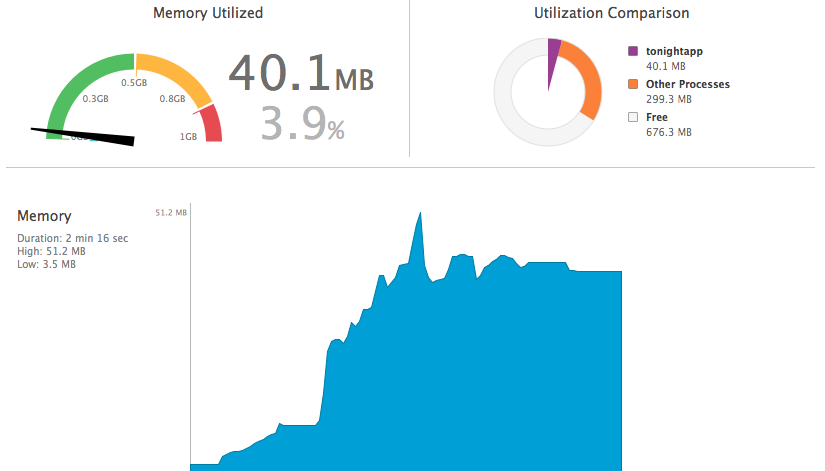
\includegraphics[width=0.9\textwidth]{Images/iosMem}
			\caption{Memory usage during operation}
			\label{fig:iosMem}
		\end{minipage}%
		\begin{minipage}{.5\linewidth}
			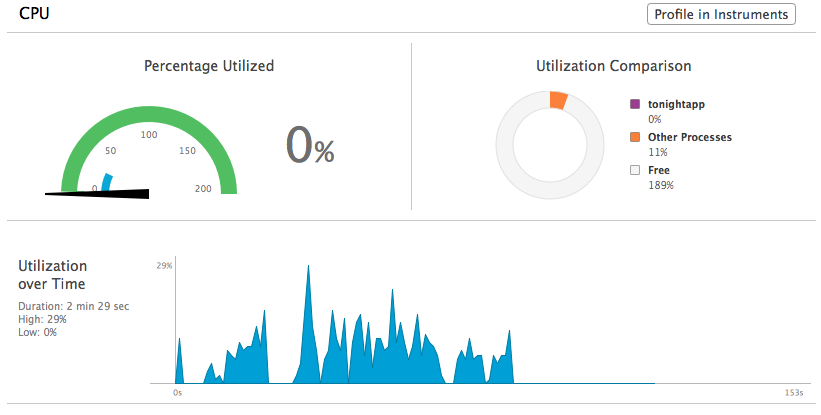
\includegraphics[width=0.9\textwidth]{Images/iosCPU}
			\caption{CPU usage during operation}
			\label{fig:iosCPU}
		\end{minipage}
		\label{fig:iosResources}
	\end{figure}

\section{Integration Testing}
	As the project was developed in the various different features, and tested inside of these features a big bang approach was taken for the integration testing. To do this I first built the sections and then using the development server option of Rails I set up a job and ran the rake task to pull in the event data for the job that was specified. This all worked without any issues, it pulled the data into the correct place and followed the right rules set by the job definition stored in the database. 

	Integration testing between the mobile application and server application was completed by checking that the application receives the events and parses these correctly into the views. Due to the RSpec tests used to test the server application we know that the API is outputting data as expected and that the functions work as expected, therefore it's just calling these URI's and parsing the output from them. 